
\begin{titlepage}
\centering
{\Huge  陳立教育 \\}
{\Huge  2017年學科能力測驗\\}
\vspace{0.1cm}


\flushright
{\large 範圍:B1 $\sim$ B4}\hspace{0.5cm} 
%{\large 解析老師:黃弈老師}

\vspace{0.5cm}

\fbox{ \parbox{\textwidth}{
        \begin{center}
            {\Huge 作答注意事項}
        \end{center}
        考試時間:100分鐘\\
        
        作答方式:
        \begin{minipage}[t]{15cm}
            \begin{itemize}
            \item 選擇(填)題用 2B 鉛筆在「答案卡」上作答;更正時,應以橡皮擦擦拭,切勿使用修正液(帶)。
            \item 非選擇題用筆尖較粗之黑色墨水的筆在「答案卷」上作答;更正時,可以使用修正液(帶)。
            \item 未依規定畫記答案卡,致機器掃描無法辨識答案;或未使用黑色墨水的筆書寫答案卷,致評閱人員無法辨認機器掃描後之答案者,其後果由考生自行承擔。
            \item 答案卷每人一張,不得要求增補。
            \end{itemize}
        \end{minipage}
        \vspace{1cm}
        
        選填題作答說明:
        \begin{minipage}[t]{14cm}
                 選填題的題號是A,B,C,……,而答案的格式每題可能不同,考生必須依各題的格式填答,且每一個列號只能在一個格子畫記。請仔細閱讀下面的例子。 \\
                 
                     例:若第B題的答案格式是 $\underline{\ \FR{\textcps{18}}{\textcps{19}}\ }$,而依題意計算出來的答案是$\FR{3}{8}$ ,則考生必須分別在答案卡上的第$18$列的 3 與第$19$列的 8 畫記,如:
                     
                     \hspace{2cm}
                         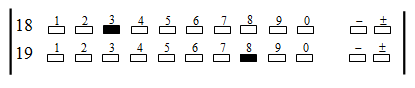
\includegraphics[width=8cm]{415x88-1.png} \\
                     
                     \vspace{0.5cm}
                     例:若第C題的答案格式是 $\underline{\ \FR{\textcps{20}\textcps{21}}{50}\ }$,而答案是 $\FR{-7}{50}$ 時,則考生必須分別在答案卡的第$20$列的 - 與第$21$列的 7 劃記,如:
                     
                         \hspace{2cm} 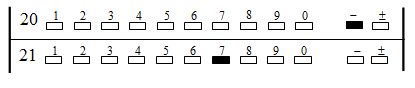
\includegraphics[width=8cm]{415x88-2.png} \\
                     
        \end{minipage} 
        }}\\
\vspace{1cm}
%下方補習班通訊方式
\begin{flushleft}
    \small
        \begin{tabular}{llll}
         {\HWHH 台中總部}:& 台中市北區三民路三段125號 1 樓  & 04-22270156 &【全新教學旗艦中心。光南大批發旁】\\
         {\HWHH 豐原分部}:& 台中市豐原區中正路33號6F		  & 04-25130567 &【豐原火車站旁,諾貝爾書局正對面大樓】
        \end{tabular}
    \end{flushleft}
\end{titlepage}
